Two main experiments have been conducted; the first experiment involves applying the aforementioned machine learning methods on the feature extracted vector. The second experiment involves applying deep learning practices on the raw image data. 

\subsection*{Experiment 1: Machine Learning}
The machine learning experiments are implemented in Python 3 using the SciKit Learn \cite{scikit-learn}, except the Neural Network that are implemented in Keras \cite{chollet2015keras} using Tensorflow \cite{tensorflow2015-whitepaper} backend. \\

All classifiers have been run on the FIN-Benthic data set and on the FIN-Benthic concatenated data set using Grid Search and CV to find the best hyperparameters, except the neural networks. As grid search has been used to find the best set of parameters for each of the classifiers and on the different data sets, it has not given the same results for best hyperparameter settings. Only the best performing setting of hyperparameters for each classifier are presented in this paper.

\begin{figure}[H]
    \centering
    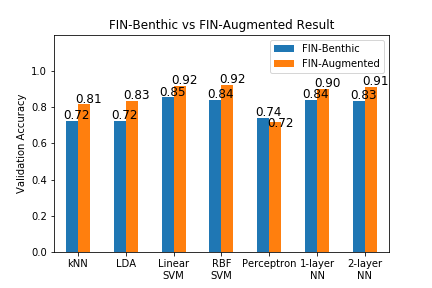
\includegraphics[width=0.5\textwidth]{figures/fin-benthic-same.png}
    \ContinuedFloat
    \caption[]{The best setting for each of the classifiers in terms of accuracy. Generally the classifiers perform best on the concatenated data set. The assumption about concatenating the pair sample of the same bug holds true.}
    \label{fig:fin_ben_concat}
\end{figure}

I added PCA to the classification pipeline and ran the same grid search on all the classifiers on both data sets. For all runs the dimensionality have been reduced to $n=\{128, 256, 512, 1024\}$ principal components. PCA add additional time to the pipeline, however the time to train and predict on fewer dimensions significantly improved. Although the dimensionality have been reduced with a large margin it does not have huge impact on the classification accuracy for all classifiers.
The ones that showed the largest improvements was kNN and LDA.

\begin{figure}[H]
    \centering
    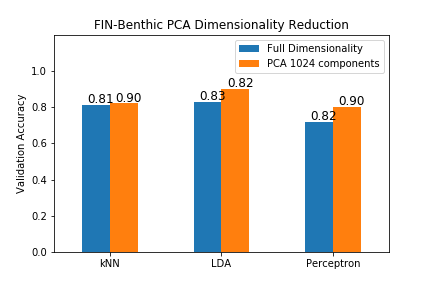
\includegraphics[width=0.5\textwidth]{figures/pca_improvement.png}
    \ContinuedFloat
    \caption[]{Adding PCA 1024 components to the pipeline improves classification accuracy by 5 point for kNN and 11 points for LDA. The other classifier showed similar results to full dimensions. The two improved classifiers seems to more prone to noise, thus PCA shows these big improvements. However PCA might still be useful for the other classifiers as it reduces training time by a large margin.}
    \label{fig:pca_improve}
\end{figure}

I did the same procedure for the augmented data set. 

\begin{figure}[H]
    \centering
    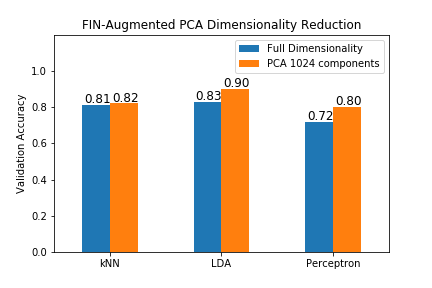
\includegraphics[width=0.5\textwidth]{figures/pca__concat_improvement.png}
    \ContinuedFloat
    \caption[]{Adding PCA 1024 components to the pipeline improves classification accuracy by 1 point for kNN, 7 points for LDA and 8 points for the Perceptron. The other classifier showed similar results to full dimensions. It seems the perceptron is better as discriminating the reduced version of the augmented data set. The PCA transformation seems to give more linearly separable features.}
    \label{fig:pca_concat_improve}
\end{figure}

\subsection*{Experiment 2: Deep Learning}

I set up an InceptionResNetV2 and initialized it with pre-trained ImageNet weights. The input layer i changed to equal the image size, and I added a softmax classifier equivalent to the number of classes i.e. 29. I used data augmentation to generate artificial samples and counter avoid overfitting. I trained the network for 100 epochs, but was not able to get validation accuracy above 0.80. Unfortunately due to limited access to GPUs, I could not do several runs to perfection the hyperparameter and augmentation to obtain higher accuracy. 
